\documentclass[border=5mm]{standalone}
\usepackage{tikz} 
\usetikzlibrary{positioning,arrows.meta,quotes}
\begin{document}
% latent variable model
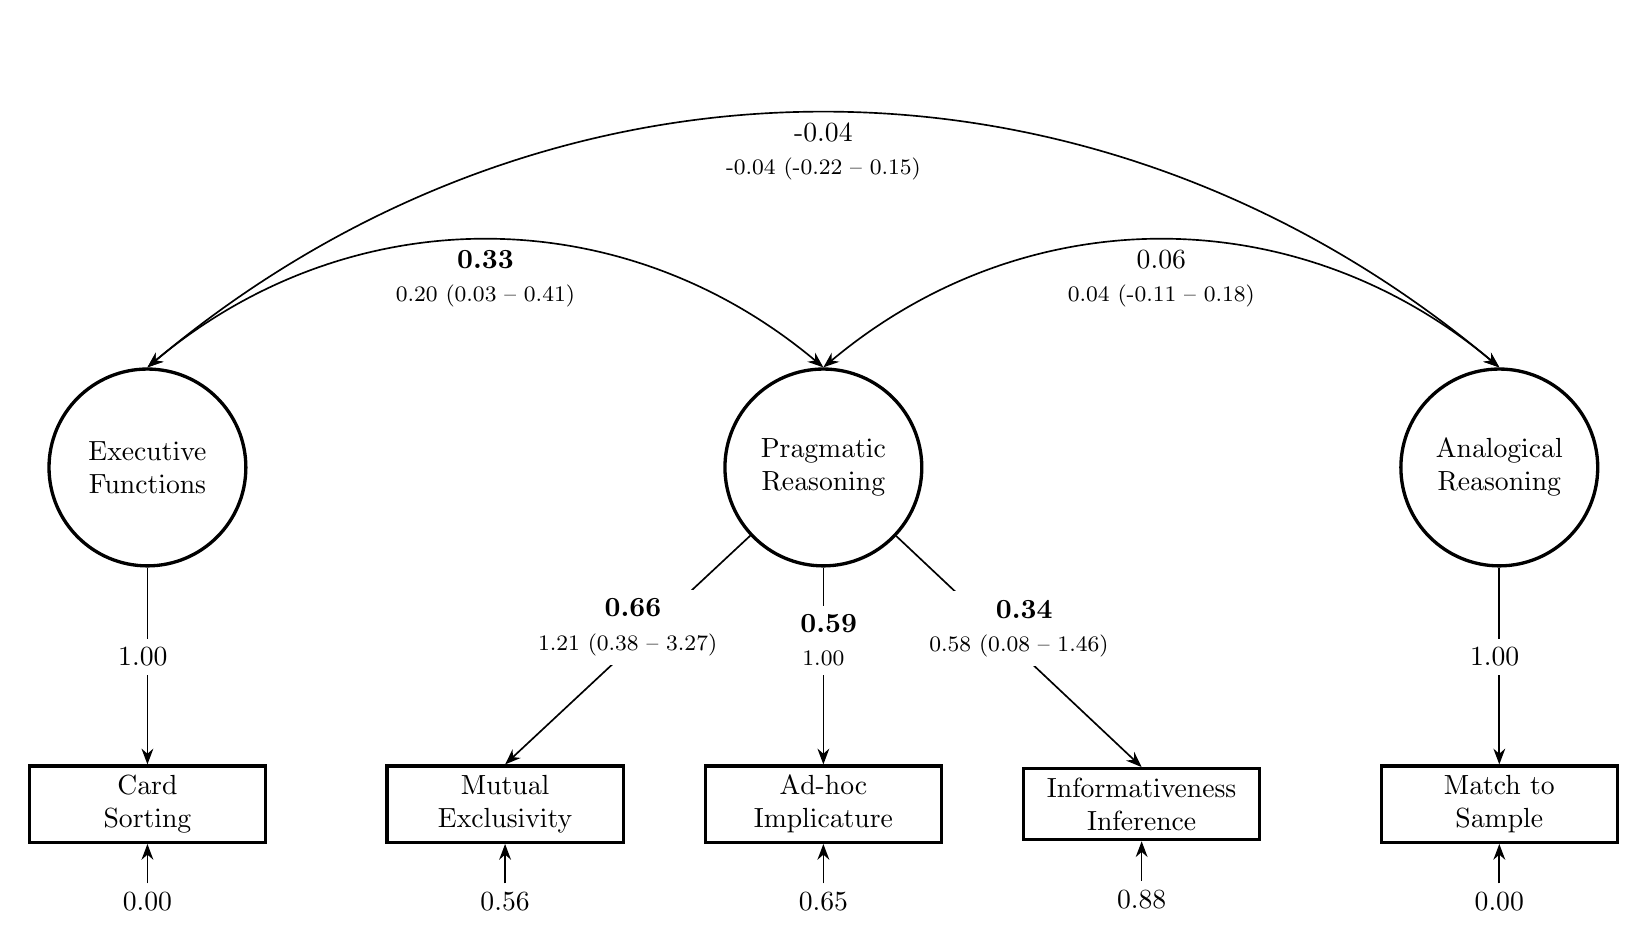
\begin{tikzpicture}[
  transform shape, node distance=0cm,
  roundnode/.style={circle, draw=black, very thick, minimum size=2.5cm},
  squarednode/.style={rectangle, draw=black, very thick, minimum width=3cm},
  arrow/.style = {semithick,-Stealth},
  path/.style = {semithick,-Stealth},
  dotnode/.style={fill,inner sep=0pt,minimum size=2pt,circle} % <- this is new
]

%Nodes
\node[roundnode,  align=center] (prag) {Pragmatic \\ Reasoning};
\node[squarednode, align=center,below=2.5cm of prag,xshift=0cm] (X2) {Ad-hoc \\ Implicature}; 
\node[squarednode, align=center,left=1cm of X2]    (X1) {Mutual \\ Exclusivity};
\node[squarednode, align=center,right=1cm of X2]    (X3) {Informativeness \\ Inference};

\node[squarednode, align=center,left=1.5cm of X1]    (X4) {Card \\ Sorting};
\node[squarednode, align=center,right=1.5cm of X3]    (X5) {Match to \\ Sample};

\node[roundnode, align = center, above = 2.5cm of X4] (card) {Executive \\ Functions};
\node[roundnode, align = center, above = 2.5cm of X5] (rmts) {Analogical \\ Reasoning};

%Letters
\node[below=0.5cm of X1] (e1) {0.56};
\node[below=0.5cm of X4] (e4) {0.00};
\node[below=0.5cm of X5] (e5) {0.00};
\node[below=0.5cm of X2] (e2) {0.65};
\node[below=0.5cm of X3] (e3) {0.88};
%\node[left=1cm of Xk] (ek) {$e_k$};
%
%%Arrows
\draw[arrow] (prag) -- node[align = center, fill=white, anchor=base] {\textbf{ 0.66} \\ \footnotesize{1.21 (0.38 -- 3.27)}} (X1.north);
\draw[arrow] (prag) -- node[align = center,fill=white, anchor=base] {\textbf{ 0.59} \\ \footnotesize{1.00 }} (X2.north);
\draw[arrow] (prag) -- node[align = center,fill=white, anchor=base] {\textbf{ 0.34} \\ \footnotesize{0.58 (0.08 -- 1.46)}} (X3.north);

\draw[arrow] (card) -- node[align = center,fill=white, anchor=base] {1.00 } (X4.north);
\draw[arrow] (rmts) -- node[align = center,fill=white, anchor=base] {1.00 } (X5.north);


% Correlations

\draw [>=Stealth, semithick, <-> ] (prag.north) to ["\textbf{0.33} \\ \footnotesize{0.20 (0.03 -- 0.41)}"align = center, out=140,in=40] (card.north);
\draw [>=Stealth, semithick, <-> ] (rmts.north) to ["0.06 \\ \footnotesize{0.04 (-0.11 -- 0.18)}" align = center, out=140,in=40] (prag.north);
\draw [>=Stealth, semithick, <-> ] (rmts.north) to ["-0.04 \\ \footnotesize{-0.04 (-0.22 -- 0.15)}" align = center, out=140,in=40] (card.north);



%
\draw[arrow] (e1) -- (X1);
\draw[arrow] (e2) -- (X2);
\draw[arrow] (e3) -- (X3);
\draw[arrow] (e4) -- (X4);
\draw[arrow] (e5) -- (X5);
%\draw[arrow] (ek) -- (Xk);





\end{tikzpicture}
\end{document}